\documentclass[tikz,border=2pt]{standalone}
\usepackage{amsmath}
\usepackage{pgfplots}
\pgfplotsset{compat=1.18}
\usetikzlibrary{arrows.meta}
\begin{document}
% Absolute risk aversion r(w) = -u''(w)/u'(w): constant alpha = 0.01 for exponential (CARA) utility,
% decreasing (1-gamma)/w = 0.5/w for power utility with gamma = 1/2; the two cross at w = 50.
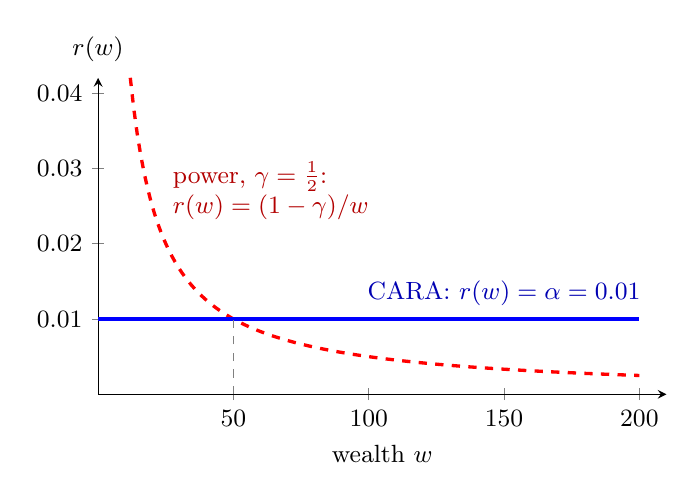
\begin{tikzpicture}[font=\small, >={Latex[length=2mm]}]
  \begin{axis}[
    axis lines=left, xmin=0, xmax=210, ymin=0, ymax=0.042,
    xtick={50,100,150,200}, ytick={0.01,0.02,0.03,0.04},
    scaled y ticks=false, yticklabel style={/pgf/number format/fixed, /pgf/number format/precision=2},
    xlabel={wealth $w$}, ylabel={$r(w)$},
    ylabel style={rotate=-90, anchor=south, at={(axis description cs:0,1.02)}},
    samples=150, width=8.8cm, height=5.6cm, clip=false]
    \addplot[red, very thick, dashed, domain=11.9:200] {0.5/x};
    \addplot[blue, very thick, domain=0:200] {0.01};
    \node[blue!70!black, anchor=south] at (axis cs:150,0.0105) {CARA: $r(w)=\alpha=0.01$};
    \node[red!70!black, anchor=west, align=left] at (axis cs:24,0.027) {power, $\gamma=\tfrac12$:\\$r(w)=(1-\gamma)/w$};
    \draw[gray, thin, dashed] (axis cs:50,0) -- (axis cs:50,0.01);
  \end{axis}
\end{tikzpicture}
\end{document}
